\documentclass[DM,lsstdraft,toc,usenatbib]{lsstdoc}

% Package imports go here
\usepackage{amsmath}	% Advanced maths commands
\usepackage{amssymb}
\usepackage{gensymb}  % degree symbol 
\usepackage{natbib}  % bibliography
\usepackage{cprotect} 
% Local commands go here

%% Journal abbreviations
%\bibliographystyle{aasjournal}

\title[Crowded fields ]{LSST  Crowded Fields photometry}

\author{
K.~Suberlak, C.~Slater,
\v{Z}.~Ivezi\'c, P.~Yoachim}

\setDocRef{LSST-2017}
\date{\today}
\setDocRevision{TBD}
\setDocStatus{draft}
\setDocAbstract{%
A report the status of crowded field photometry. We evaluate the need for performing better photometry in crowded fields by quantifying areas of the sky at a given density level. We provide an overview of density metrics, photometric methods applicable in a given stellar density regime, and recommendations for areas of improvement in the LSST Stack.}

% Change history defined here. Will be inserted into
% correct place with \maketitle
% OLDEST FIRST: VERSION, DATE, DESCRIPTION, OWNER NAME
\setDocChangeRecord{%
\addtohist{1}{2017-07-16}{First draft.}{Krzysztof Suberlak}
}

\begin{document}

% Create the title page
% Table of contents will be added automatically if "toc" class option
% is used.
\maketitle

\section{Introduction}

This is a document to report on quantifying the performance expectations and options with respect to crowded field processing.

The Large Scale Synoptic Telescope (LSST) will sample very diverse regions when it comes to stellar density, or crowdedness : from high density low-galactic latitude regions that have tens of millions of sources per square degree, to low-density regions towards the galactic poles with less than thousand sources per square degree. 

As mentioned by ~\cite{bosch2017} with regards to Hyper Suprime CAM software pipeline (based on LSST Stack, which in turn builds on the experience of the SDSS  Photo pipeline), deblending and performing a successful photometry is an inherent part of any astronomical data processing pipeline. The boundaries between deblending, measurement and detection blur in very high stellar densities, and the deeper the survey, the higher the stellar densities that it can encounter (see Sec 4.8.3 in \cite{bosch2017}). 

The way in which measurements may be affected by the crowdiness have been studied before - pilot study by ~\citep{hogg2001} confirmed the '30 beams per source' rule of thumb, albeit it depends on the source number counts (with steeper number counts we need more beams per source ). Following on that exploratory study,  ~\cite{olsen2003} describes more quantitative framework to address this issue in the era of large telescopes. 

We start with the LSST  Metrics Analysis Framework \footnote{\url{https://www.lsst.org/scientists/simulations/maf}} simulated stellar density map \footnote{\url{https://github.com/lsst/sims_maf}}, made with \verb|sims_maf/python/lsst/sims/maf/maps/createStarDensitymap.py|\footnote{\url{https://github.com/lsst/sims_maf/blob/a9bc8f6d00fae5d7ce4ff6ea7279d5a0fca29437/python/lsst/sims/maf/maps/createStarDensitymap.py}} by Peter Yoachim and Lynne Jones at UW. The dataset \verb|starDensity_r_nside_64.npz| contains 64 magnitude bins, and 49152  healpixels \footnote{see http://healpix.sourceforge.net for documentation of HEALPix}. Each pixel contains information about number of stars per square degree in a given magnitude bin.  

% WHY Southern Hemisphere  ?  
Using this data, we select magnitude bins smaller than r=24.5 in the Southern Hemisphere ($\delta < 0$).  We add stellar count across magnitude bins (selecting only  r <= 24.5 bins).   For each pixel we calculate the number of pixels that have a higher stellar count.  Since each pixel in HEALPix has an equal area, the fraction of pixel number above a certain threshold corresponds to the fraction of sky area above given density limit. See Fig.~\ref{fig:illustrate_density} for an illustration of how we define the stellar density - it is akin to a cumulative distribution. Therefore 'top 1\%' density means that only 1 in 100 pixels has a higher density than a given pixel.  Likewise,  'top 10\%' means that '10 \%' of pixels in the selected hemisphere have higher density. 

\begin{figure}
\includegraphics[width=1.0\columnwidth]{figs/Southern_sky_r_lt245_twiny.png}
%\vskip -0.15in
\caption{Illustration of how the stellar density is quantified in terms of relative pixel density. We express stellar density both in terms of number of stars per square degree (bottom axis), as well as in terms of product of sources per square arcsecond and psf effective area (upper axis )}
\label{fig:illustrate_density}
\end{figure} 


Since this definition of density includes all pixels that are within 'top 20\%', we take selection around the percentiles so that :

\begin{itemize}
\item top  1 \%  means  fraction of sky with greater density is 0.01
\item 5 \% region means such that between  4\% and 6\%
\item 20 \% region  includes   19\% - 21\%
\item 50 \% region includes 49\% - 51\% 
\end{itemize}


We illustrate the location of pixels representative of these density brackets on the sky in various projections  and coordinate systems :  cylindrical (Mercator) projection  in equatorial coordinates on Fig.~\ref{fig:cart_equat},  Mollweide projection in equatorial coordinates on Fig.~\ref{fig:mollw_equat},  and the same in galactic coordinates on Fig.~\ref{fig:mollw_galactic}. 


\begin{figure}
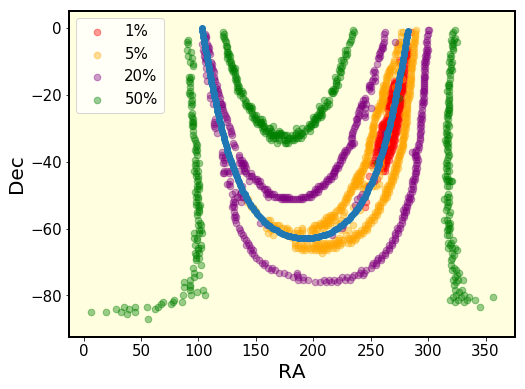
\includegraphics[width=1.0\columnwidth]{figs/Illustrate_density_regions.png}
%\vskip -0.15in
\caption{Illustration of location of regions representative of different relative density in cylindrical projection, equatorial coordinates. The blue solid line marks the location of Galactic equator. }
\label{fig:cart_equat}
\end{figure} 



\begin{figure}
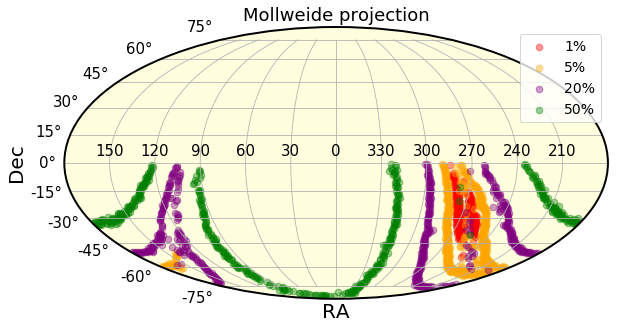
\includegraphics[width=1.0\columnwidth]{figs/Illustrate_density_regions_mollw.png}
%\vskip -0.15in
\caption{Same as Fig.~\ref{fig:cart_equat}, but in Mollweide projection, with Equatorial coordinates.}
\label{fig:mollw_equat}
\end{figure} 



\begin{figure}
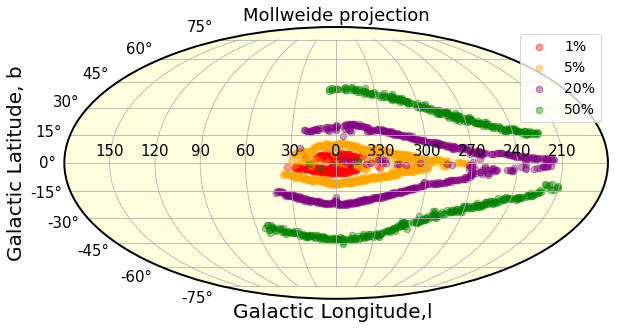
\includegraphics[width=1.0\columnwidth]{figs/Illustrate_density_regions_mollw_galactic.png}
%\vskip -0.15in
\caption{Same as Fig.~\ref{fig:mollw_equat}, but in Galactic coordinates, which emphasizes the location of regions representing different density with regards to the Milky Way. It makes sense that the highest density regions in the Southern Hemisphere ($\delta < 0$) are located close to the galactic bulge, and the decreasing density regions approximately trace the shape of our galaxy.}
\label{fig:mollw_galactic}
\end{figure} 


We compare the MAF estimates of stellar density in different density regimes to Dark Energy Camera (DECam)  data, taken with the 4-m Cerro Tololo Inter-American Observatory telescope (CTIO)\footnote{see \url{http://www.ctio.noao.edu/noao/node/1033}}. Due to inability of NOAO Data Archive \footnote{\url{http://archive.noao.edu/search/query}} query engine to handle a list of coordinates, we  first obtained all data that fulfilled very loose criteria:
\begin{itemize}
\item telescope = 'ct4m'
\item instrument = 'decam'
\item 90 sec < exposure < 125 sec 
\item release\_date < ‘2017-07-24'
\item dec < 0 
\item proctype = 'InstCal' 
\item prodtype = 'image'
\item filter is  u, g, r,  or VR 
\end{itemize}
(the SQL query used is available in the Appendix ~\ref{sec:sql_noao_decam}). 
The exposure was chosen to match the DECam data to the depth that would be achieved by LSST with 30 second exposure.  
% How was this calculated?   Ask Colin for formulaee ... 

We obtained 11928 rows fulfilling these criteria : the location of these observations on the sky, with overlaid MAF density regions , is shown on Fig.~\ref{fig:decam_regions}. 

 
\begin{figure}
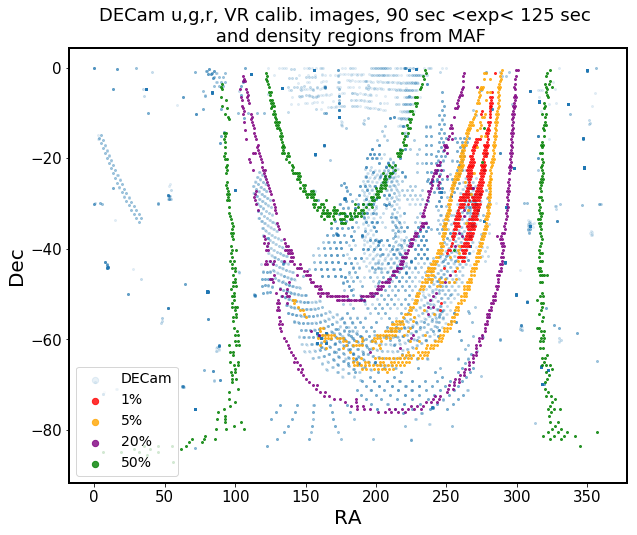
\includegraphics[width=1.0\columnwidth]{figs/Illustrate_density_regions_DECam.png}
%\vskip -0.15in
\caption{DECam observations with exposure $\in [90,125] $ sec, $\delta < 0$, taken in  u,g,r, or VR filter.  }
\label{fig:decam_regions}
\end{figure} 

We used AstroPy to match the coordinates of MAF healpixels in different density regimes to DECam imaging data. We found that of 244 top 1\% density pixels, 91 had DECam matches within 30 arcminutes, as shown on Fig.~\ref{fig:decam_matches_top}. 

\begin{figure}
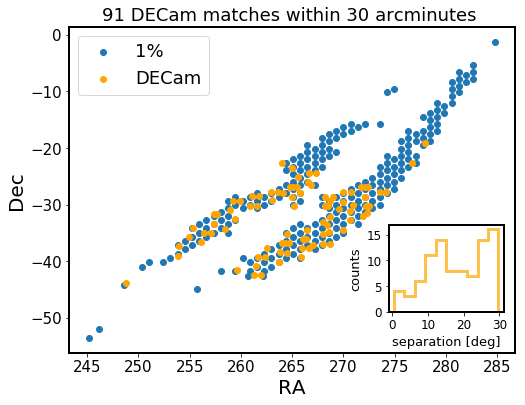
\includegraphics[width=1.0\columnwidth]{figs/Illustrate_top_1_perc_DECam_matches.png}
%\vskip -0.15in
\caption{DECam observations with exposure $\in [90,125] $ sec, $\delta < 0$, taken in  u,g,r, or VR filter, matched by 2D separation to MAF healpixels within the highest stellar density bins. The inset shows the distribution of separation between healpix coordinates and DECam image center. Each DECam image is a mosaic, and each mosaic element covers approximately 9x18 arcminutes. }
\label{fig:decam_matches_top}
\end{figure} 

We performed source extraction on ten randomly chosen DECam images that matched the coordinates of MAF pixels per given density regimen.  We used DAOStarFinder\footnote{\url{http://photutils.readthedocs.io/en/stable/photutils/detection.html}}, which includes an implementation of the DAOFIND algorithm ~\citep{stetson1987}. Since each CCD image from DECam is a mosaic, the FITS files contained 60 primary HDUs (of which the first one is opened by default in ds9). For each element of the mosaic with 2046x4094 pixels, with pixel scale of 0.27 arcsec / px , so that a single mosaic element covers an area of 0.047117 sq.deg. Using the FWHM information from the FITS header, and sigma clipped standard deviation $\sigma$, we performed source extraction with the detection threshold at $5 \sigma$ level. 

The source density scaled to the 1 square degree level is consistently an order of magnitude less than the MAF estimate. ( see table ). 

\appendix
\section{Appendix : SQL queries}

\subsection{NOAO DECam query}
\label{sec:sql_noao_decam}
\begin{lstlisting}
SELECT \
  reference, dtpropid, surveyid, release_date, start_date, \
  date_obs, dtpi, ra, dec, telescope, instrument, filter, \
  exposure, obstype, obsmode, proctype, prodtype, seeing, \
  depth, dtacqnam, filesize, md5sum, \
  reference AS archive_file
FROM \
  voi.siap \
WHERE \
  ((exposure > 90) AND (exposure <125 ) )  \
AND release_date < '2017-07-24' \
AND (dec <= 0) \
AND (proctype = 'InstCal') \
AND (prodtype = 'image') \
AND (telescope = 'ct4m') \
AND (instrument = 'decam') \
AND ((filter ILIKE 'u DECam%' ) \
OR (filter ILIKE '%g DECam%' ) \
OR (filter ILIKE '%r DECam%' ) \
OR (filter ILIKE '%VR DECam%' ) ) \
ORDER BY date_obs ASC LIMIT 250000
\end{lstlisting}

%%%%%%%%%%%%%%%%%%%%%%%%%%%%%%%%%%%%%%%%%%%%%%%%%%
%%%%%%%%%%%%%%%%%%%% REFERENCES %%%%%%%%%%%%%%%%%%
%%%%%%%%%%%%%%%%%%%%%%%%%%%%%%%%%%%%%%%%%%%%%%%%%%

\bibliographystyle{apj}
\bibliography{references}
\end{document}